Nous allons parcourir notre arbre des features selon la méthodologie Depth First Search.

\begin{description}

\item [LocalSharingEconomy]
\underline{Déf. :}  Une économie d'échange local est un système organisé dont l'objectif principal est de promouvoir des échanges de biens et/ou de services dans une zone géographique limitée.  Par exemple,  BuurtPensioen favorise les échanges locaux via l'adhésion à une branche.  Par contre,  lystème des SEL est un système centralisé auquel des communes peuvent s'inscrire.   
\\ \underline{Justif. :}  Ce feature est la racine de l'arbre,  ne pas l'inclure signifierait que l'organisation analysée ne peut pas correspondre à l'analyse proposée ici.
\newline

\item [ModèleEconomique]
\underline{Déf. :}  Le modèle économique d'une économie d'échange local correspond aux caractéristiques de l'organisation telle qu'elle est vécue,  indépendamment de l'outil utilisé.
\\ \underline{Justif. :}  Ce feature est obligatoire car toute analyse d'une économie d'échange local doit être d'abord décrite avant de pouvoir s'intéresser à l'outil.
\newline

Nous arrivons maintenant dans le premier sous-arbre : \textbf{PublicCible}.
\newline
\begin{center}
\fbox{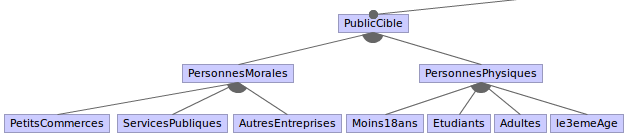
\includegraphics[scale=0.5]{PublicCible.png}}
\end{center}

\item [PublicCible]
\underline{Déf. :}  Le public cible d'une économie d'échange local correspond aux acteurs autorisés à participer aux échanges dans l'organisation.
\\ \underline{Justif. :}  Ce feature est obligatoire car l'organisation n'a pas de sens s'il n'y a pas d'acteurs définis.  Ainsi,  il est obligatoire de sélectionner au moins 1 des fils mais il peut en avoir de plusieurs types.  
\newline

\item [PersonnesMorales]
\underline{Déf. :}  Une personne morale est une construction juridique.  On place dans cette catégorie d'acteurs toutes les entités,  institutions,  organisations et autres groupes considérés comme des acteurs du système.  
\\ \underline{Justif. :}  Certaines organisations permettent,  par exemple,  à des entreprises de faire des échanges entre elles.  Il peut aussi s'agir d'acteurs du service public.  La distinction entre personne morale et physique est nécessaire car cela pourra avoir des répercutions sur l'outil utilisé d'une part pour les fonctionnalités accessibles et d'autre part pour la représentation des données.  Ainsi,  une personne physique pourrait être identifiée par ses nom,  prénom et date de naissance tandis qu'une personne morale ne requièrerait qu'une dénomination générale. 
\newline

Parmi les personnes morales,  on distingue les \textbf{petits commerces},  les \textbf{services publics} et les \textbf{autres entreprises}.

\item [PetitsCommerces]
\underline{Déf. :}  Ce feature regroupe les personnes morales de type privé et de petite taille (PME,  indépendants,  \dots )
\\ \underline{Justif. :}  Etant donné la visée géographique des systèmes d'échange local,  il est tout à fait envisageable qu'une organisation permette,  par exemple,  aux artisans locaux de participer aux échanges.  
\newline

\item [ServicesPublics]
\underline{Déf. :}  Les services publics sont toutes les institutions reconnues juridiquement comme agissant pour l'intérêt général.
\\ \underline{Justif. :}  Des institutions publiques locales peuvent être impliqués dans l'oganisation.  Par exemple,  une commune pourrait faire un appel aux volontaires pour participer à une campagne de nettoyage de la commune.  
\newline

\item [AutresEntreprises]
\underline{Déf. :}  Certains acteurs d'un système d'échange peuvent ne pas être des petits commerces ni services publics.  Par exemple,  une multinationale qui désire insérer sa filiale locale dans l'organisation.
\\ \underline{Justif. :}  Ce feature permet de prendre en compte les acteurs qui ne seraient pas repris dans les cas pré-cités.  
\newline

\item [PersonnesPhysiques]
\underline{Déf. :}  Une personne physique est un être humain.
\\ \underline{Justif. :}  Dans la pratique,  beaucoup d'organisations sont composées en très grande majorité de personnes physiques.  Mais il convient de faire une distinction parmi celles-ci car  l'outil peut varier  selon le type de personnes visées.
\newline

Parmi les personnes physiques,  on distingue les différentes tranches d'âge : \textbf{Moins18ans}, \textbf{Etudiants}, \textbf{Adultes}, \textbf{le3emeAge}.


\item [Moins18ans]
\underline{Déf. :}  Ce feature représente la possibilité à des personnes de moins de 18 ans d'être acteurs dans l'organisation.
\\ \underline{Justif. :}  Ce cas est à prendre en considération car si des personnes mineures aux yeux de la loi peuvent intégrer le système,   il se peut qu'il faille adapter l'outil pour éviter toute dérive.
\newline

% ================= 10 ===========
\item [Etudiants]
\underline{Déf. :}  Ce feature représente la possibilité aux étudiants d'être acteurs dans l'organisation.
\\ \underline{Justif. :}  Cibler les étudiants (jeunes) dans l'organisation peut être lié à diverses raisons.  D'abord,  le système peut être destiné aux jeunes.  Mais aussi,  il se pourrait que l'organisation,  telle que BuurtPensioen,  favorise les liens intergénérationnels.
\newline

\item [Adultes]
\underline{Déf. :}  Ce feature reprend la plus grand emajorité de la population.
\\ \underline{Justif. :}  Au même titre que les étudiants,  les adultes peuvent être une cible du système si,  par exemple,  on désire favoriser l'intergénérationnel.
\newline

\item [le3emeAge]
\underline{Déf. :}   On désigne ici un public plus âgé.  Ce public peut englober différents profils : les personnes retraitées,  à mobilité réduire due à l'âge,  \dots 
\\ \underline{Justif. :}  Un système tel que BuurtPensioen place ce feature au centre se objectifs puisqu'il s'agit,  tel que expliqué dans la description du problème,  d'un système de pensions entre voisins.  Le 3ème âge est donc un public privilégié et influe,  par exemple,  sur l'ergonomie de l'outil.
\newline

Ceci termine notre premier sous-arbre dont l'objectif était de décrire le ou les public(s) cible(s) du modèle économique.  La second partie que nous allons voir concerne la \textbf{monnaie} utilisée au sein du système.

\begin{center}
\fbox{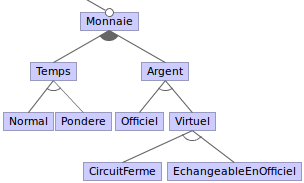
\includegraphics[scale=0.5]{Monnaie.png}}
\end{center}

\item [Monnaie]
\underline{Déf. :}  La monnaie utilisée dans une économie d'échange local est le moyen utilisé pour quantifier la valeur d'un bien ou un service.  Dans le dictionnaire des termes ( \ref{dicoMonnaie} ),  le principe de la monnaie a déjà été expliqué.   Ce feature englobe donc les différentes possibilités de monnaie.
\\ \underline{Justif. :}  Ce feature est optionnel car il se peut qu'une organisation n'utilise pas de monnaie.  Nous aurions alors un système d'échange gratuit.  Ceci existe déjà que ce soit pour des biens (les "donneries") ou services.  Si une monnaie est utilisée,  alors le système se limite à une seule.  Il est possible qu'une organisation aie plusieurs monnaies mais pour limiter la complexité de l'analyse et du framework,  nous nous limiterons au cas ou l'organisation utilise 0 ou 1 monnaie pour les échanges.
\newline

\item [Temps]
\underline{Déf. :}  Certaines organisations utilisent le temps comme monnaie d'échange.  La quantité est définie en unités temporelles habituelles (minutes,  heures,  jours, \dots ).  
\\ \underline{Justif. :}  Attention,  choisir cette monnaie comme moyen d'échange a un impact sur les possibilités futures d'échange.  En effet,  ce feature est à rejeter si l'on désire pouvoir échanger des biens/objets car utiliser cette monnaie représente du temps passé par une personne à réaliser une action.  Cela n'a donc pas de sens d'attribuer cette unité à un objet.
\newline

\item [Normal]
\underline{Déf. :}  Le temps peut être utilisé comme monnaie en représentant simplement le temps passé à réaliser le service échangé.
\\ \underline{Justif. :}  La plupart des organisations utilisant le temps comme monnaie d'échange pour des services se limitent à ce feature-ci.
\newline

\item [Pondéré]
\underline{Déf. :}  Ce feature laisse la possibilité à une organisation de personnaliser sa notion du temps.  Par exemple,  en considérant que certains services rapportent 2 fois le temps passé par la personne car celui-ci est plus rare.  
\\ \underline{Justif. :}  Ce feature n'est pas issu d'un constat de réalité mais plutôt d'une ouverture vers de nouvelles possibilités pour le futur.
\newline

\item [Argent]
\underline{Déf. :}  Ce feature désigne les monnaies plus classiques qui peuvent prendre une forme plus matérielle que le temps,  ou bien n'être que des monnaies virtuelles.
\\ \underline{Justif. :}  Ce feature est obligatoire si l'on désire pouvoir échanger des objets.  
\newline

\item [Officiel]
\underline{Déf. :}  Les monaies officielles regroupent,  tel que le nom l'indique,  les monnaies reconnues par des institutions publiques et englobent l'euro,  le dollar,  \dots.  
\\ \underline{Justif. :}  Pour des organisations désirant rester proches du système économique occidental "classique",  les monnaies officielles sont une évidence même.
\newline

\item [Virtuel]
\underline{Déf. :}  Les monnaies virtuelles englobent,  par opposition aux monnaies officielles,  les autres types d'argent qui peuvent exister mais ne seraient pas reconnues par des institutions publiques ou bien uniquement de façon très locale et dans un usage restreint.
\\ \underline{Justif. :}  Les systèmes d'échange local font partie des alternatives au système économique actuel qui a tendance à uniformiser et globaliser,  entre autres,  l'argent.  Il n'est donc pas rare de rencontrer des organisations qui ont créé leur propre monnaie complémentaire.  
\newline

% ================= 20 ===========
\item [CircuitFerme]
\underline{Déf. :}  Parmi les monnaies complémentaires,  certaines sont prévues pour ne pas être échangées afin,  par exemple,  de garder un aspect très local.  
\\ \underline{Justif. :}  
\newline

\item [EchangeableEnOfficiel]
\underline{Déf. :}  A l'inverse,  certaines monnaies peuvent être échangées contre de l'argent officiel.
\\ \underline{Justif. :}  Il est possible de déveloper un système de monnaie alternative (points ou autres) pour les échanges en interne et ceux-ci et de pouvoir les échanger auprès de l'organisation contre de l'argent réel.
\newline

\begin{center}
\fbox{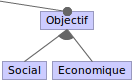
\includegraphics[scale=0.5]{Objectif.png}}
\end{center}

\item [Objectif]
\underline{Déf. :}  Ce feature doit être inclu afin de définir quel est l'objectif du modèle économique étudié.
\\ \underline{Justif. :}  Il est obligatoire de définir le ou les objectifs car cela peut avoir un impact sur l'outil final.  Plusieurs objectifs sont compatibles mais il en faut au moins 1.
\newline

\item [Social]
\underline{Déf. :}  Une organisation qui a pour but d'améliorer le bien-être des gens a un but social.
\\ \underline{Justif. :}  Beaucoup d'organisations actuelles ont princpalement un but social (ex. BuurtPensioen).
\newline

\item [Economique]
\underline{Déf. :}  Une organisation qui désire faire du profit grâce à l'orgnisation des échanges a un but économique.
\\ \underline{Justif. :}  Pour rendre ce genre de système rentable,  plusieurs exemples sont possibles : faire payer un abonnement aux utilisateurs,  faire payer chaque ou certains échanges, \dots
\newline

\item [Outil]
\underline{Déf. :}  Après avoir analysé le modèle économique du système d'échange local,  nous allons passer à l'outil.  On désigne ici les moyens matériels utilisés pour gérer l'économie locale.  Ce feature est optionnel car il est possible d'analyser un système sans que celui-ci ne possède d'outil.  
\\ \underline{Justif. :}  Le feature est à inclure si l'organisation possède un quelconque outil de gestion matérialisé,  c'est-à-dire au minimum sous forme papier.
\newline

\begin{center}
\fbox{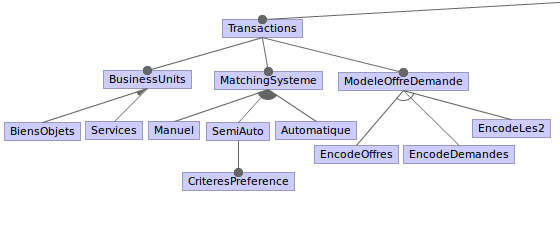
\includegraphics[scale=0.5]{Transactions.png}}
\end{center}

\item [Transactions]
\underline{Déf. :}  Les transactiosn sont les échanges possibles au sein de l'organisation.
\\ \underline{Justif. :}  Ce feature est obligatoire car si le système possède un outil de gestion,  le but premier de celui-ci sera de gérer les échanges entre acteurs.
\newline

\item [BusinessUnits]
\underline{Déf. :}  Les BusinessUnits représentent les unités échangées dans le système.
\\ \underline{Justif. :}  Ce feature est obligatoire car pour qu'il y ait échange,  il faut qu'il y ait quelque chose à échanger.
\newline

2 types d'unités sont échangeables : les \textbf{Biens ou Objet}s,  et les \textbf{Services}

\item [BiensObjets]
\underline{Déf. :}  Les biens ou objets sont des choses perceptibles par la vue et le toucher \footnote{\href{http://www.larousse.fr/dictionnaires/francais/objet/55366}{http://www.larousse.fr/dictionnaires/francais/objet/55366}}  et qui,  dans notre cas,  peuvent changer de propriétaire.
\\ \underline{Justif. :}  Ce feature est à inclure si l'outil permet l'échange d'objets matérialisés. 
\newline

\item [Services]
\underline{Déf. :}  Un service est un travail manuel ou intellectuel réalisé par une personne pour aider une ou plusieurs autres personnes.  Exemples de services : tâches ménagères,  jardinage,  baby-sitting,  \dots .
\\ \underline{Justif. :} Ce feature est à inclure si 'lorganisation permet l'échange de services entre les acteurs. 
\newline

% ================= 30 ===========
\item [MatchingSysteme]
\underline{Déf. :}  Le système de matching correspond aux fonctionnalités qui permettent de retrouver une offre lorsqu'on fait une demande ou vice-versa.  Les 3 possibilités de matching sont,  à chaque fois,  un choix à faire entre laisser plus de possibilités à l'utilisateur de choisir mais alors la recherche prend plus de temps,  ou à l'inverse,  accélérer la recherche pour l'utilisateur mais cela signifie lui laisser moins de choix.
\\ \underline{Justif. :}  Tous les systèmes d'échange local possèdent un système de matching qui sera,  pour le cas le moins automatisé,  totalement manuel.  Plusieurs systèmes peuvent cohabiter au sein du même système.
\newline

\item [Manuel]
\underline{Déf. :}  Un matching manuel signifie que les acteurs des échanges consultent et acccèdent à une liste des offres et/ou demandes manuellement,  sans qu'un tri préalable ait été effectué par l'outil.
\\ \underline{Justif. :} Ce feature est le fonctionnement le plus simple et celui laissant le plus de possibilités de choix aux acteurs. 
\newline

\item [Semi-auto]
\underline{Déf. :}  Un matching semi-automatique signifie que l'acteur qui désire effectuer une recherche dans les transactions encodées dans le système,  recevra une liste épurée de concordancees.  Cette liste est générée par le système sur base d'un ou plusieurs critères de préférence.
\\ \underline{Justif. :}  Ce feature offre moins de choix à l'utilisateur mais accélère la recherche d'une correspondance.
\newline

\item [Critère]
\underline{Déf. :}  Un critère de préférence correspond à un argument qui sera utilisé par le système pour effectuer un tri parmi toutes les possibilités de correspondance.
\\ \underline{Justif. :}  Un matching semi-automatique doit avoir au moins 1 critère sur lequel effectuer le tri de base.  Ce critère est lié à ce qui est recherché,  c'est-à-dire un bien ou un service,  ou à la transaction plus généralement.  Par exemple,  la date à laquelle un service doit avoir lieu peut être un critère de préférence ou bien,  pour toute transaction,  la distance à parcourir pour obtenir l'objet / réaliser la tâche,  peut également être un critère de préférence.   
\newline

\item [Automatique]
\underline{Déf. :}  Un matching automatique correspond à la fonctionnalité où le système recherche lui-même une correspondance dans les offres ou demandes enregistrées dans le système.  L'acteur n'a alors qu'une seule possibilité de correspondance.  Les critères utilisés pour faire correspondre les transactions sont internes au système.
\\ \underline{Justif. :}  Ce feature amène un système très efficace mais très peu tolérant des exigences des utilisateurs.  
\newline

\item [ModeleOffreDemande]
\phantomsection
\label{featOD}
\underline{Déf. :}  Le modèle d'offre et demande correspond aux fonctionnalités présentes dans l'outil pour faire savoir au système que l'on recherche ou que l'on propose un bien ou un service.  Par exemple,  les sites de type eBay,  2ememain et autres,  ne permettent l'encodage que des offres.  Si un utilisateur désire acquérir un objet,  il n'a pas la possibilité d'encoder sa recherche dans le site,  il doit chercher et essayer de trouver ce qui correspond le mieux à ses besoins.  Ce feature représente les actions possibles pour un acteur du système (enregistré ou non,  administrateur ou non,  à voir selon les autres features décrits ci-après).  
\\ \underline{Justif. :}  Ce feature est important à définir car l'outil peut être tout à fait différent selon les possibilités offertes aux acteurs.  Par facilité pour l'élaboration des contraintes décrites plus loin,  3 features sont disponibles mais 1 seul peut être choisi.  Soit on encode les offres,  soit les demandes,  soit les 2.  Cette notation remplace une cardinalité de 1 ou + avec 2 éléments possibles mais ne change pas sa signification.
\newline

\item [EncodeOffres]
\underline{Déf. :}  Encoder les offres implique que l'acteur d'une transaction puisse insérer dans le système une description du bien ou service qu'il est prêt à échanger avec un autre acteur.  Conformément à la définition donnée,  l'acteur se trouve alors dans la position du fournisseur (\ref{dicoTermes}).
\\ \underline{Justif. :}  Beaucoup de sites de commerce en ligne fonctionnent de la sorte ( \href{http://www.befr.ebay.be/}{eBay\copyright} et autres )
\newline

\item [EncodeDemandes]
\underline{Déf. :}  Encoder les demandes implique que l'acteur d'une transaction puisse insérer dans le système une description du bien ou service qu'il aimerait pouvoir obtenir d'un autre acteur.   Celui-ci serait donc dans la position de bénéficiaire ( \ref{dicoTermes}).
\\ \underline{Justif. :}  
\newline

\item [EncodeLes2]
\underline{Déf. :}  Les 2 possibilités précitées peuvent coexister dans un même système.
\\ \underline{Justif. :}  Feature à inclure si le système offre les 2 possibilités expliquées ci-dessus.
\newline

\begin{center}
\fbox{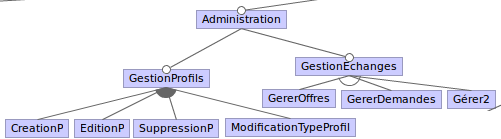
\includegraphics[scale=0.5]{Administration.png}}
\end{center}

\item [Administration]
\underline{Déf. :}  L'existence d'un système d'administration permet d'accéder à des fonctionnalités avancées de l'outil qui ne sont pas accessibles aux utilisateurs.
\\ \underline{Justif. :}  Beuacoup d'outils ont une possibilité d'administration mais ce n'est pas une obligation.  Le feature est donc optionnel.  De plus,  les 2 sous-arbres sont optionnels car ils représentent une modification des données du système mais des outils pourraient avoir des fonctionnalités d'administration plus orientées "technique" (modification du texte de description dans une page, \dots).
\newline

% ================= 40 ===========
\item [GestionProfils]
\underline{Déf. :}  Une des fonctionnalités administratives peut être la gestion des comptes d'utilisateurs.
\\ \underline{Justif. :}  Inclure ce feature signifie qu'il est possible de modifier les données qui présentent les acteurs dans le système.
\newline

\item [CreationP - EditionP - SuppressionP]
\underline{Déf. :}  La création/modificiation/suppression d'un profil permet à un administrateur d'enregistrer/supprimer lui-même une personne dans le système ou de modifier ses informations.
\\ \underline{Justif. :}  Certains outils restreignent l'inscription à une personne physique elle-même,  par exemple,  via l'utilisation d'un lecteur de carte d'identité électronqiue pour éviter les comptes anonymes.  La fonctionnalité de création ou modification via l'administration peut donc être disponible,  ou pas.  La suppression peut aussi ne pas être autorisée si on désire que les utilisateurs gardent un seul et même compte "pour toujours". 
\newline

\item [ModificationTypeProfil]
\phantomsection
\label{featTypes}
\underline{Déf. :}  Certains outils exigent que les membres fassent partie de différents types de profil.  Par exemple,  dans BuurtPensioen,  il existe un système de "membre vérifié".  Les acteurs qui s'inscrivent sont d'abord du type "non-vérifié" et suite à quelques démarches administratives et données particulières encodées,  ils peuvent accéder au statut de "vérifié".  
\\ \underline{Justif. :}  Ce feature n'a de sens que si le système de types de profils (voir features Utilisateurs \ref{featUtils}).
\newline

\item [GestionEchanges]
\underline{Déf. :}  Une fonctionnalité importante de l'administration peut concerner des modifications sur les offres ou demandes encodées dans le système.
\\ \underline{Justif. :}  Tout comme pour la gestion des profils,  il est possible que l'on offre pas la possibilité de les biens ou services que les utilisateurs ont encodés.  Ce feature est donc optionnel.  S'il est présent,  alors 1 seul des 3 sous-arbre est possible.  Il s'agit du même pattern que pour le modèle des offres et demandes ( \ref{featOD} ).
\newline

\item [GérerOffres - GérerDemandes - Gérer2]
\underline{Déf. :}  Cette gestion peut concerner l'ajout/suppression d'offres ou demandes ainsi que de la modification des données relatives.  
\\ \underline{Justif. :}  Un exemple d'utilité à cette fonction est simplement la surveillance des annonces faites dans l'outil afin d'éviter les dérives telles que les arnaques ou trafics d'objets volés,  \dots .   
\newline

Nous allons maintenant analyser les fonctionnalités qui peuvent êtres offertes par un système de gestion des utilisateurs enregistrés.

\begin{center}
\fbox{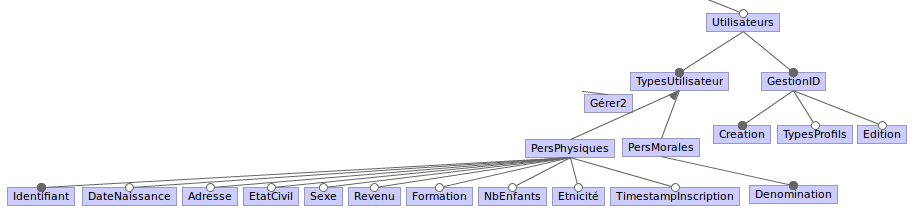
\includegraphics[scale=0.5]{Utilisateurs.png}}
\end{center}

\item [Utilisateurs]
\phantomsection
\label{featUtils} 
\underline{Déf. :}  Certains outils proposent aux acteurs des transactions de s'enregistrer dans l'outil,  par exemple,  via la création d'un compte ou profil unique.  
\\ \underline{Justif. :}  Même si beaucoup d'outils intègrent cette fonctionnalité,  ce feature est optionnel car un système d'échange peut tout à fait fonctionner sans que les acteurs n'aient la possibilité de s'enregistrer.  Par exemple,  le système de donnerie \footnote{\href{https://luna.agora.eu.org/listes/cgi-bin/mailman/listinfo/donnerie}{https://luna.agora.eu.org/listes/cgi-bin/mailman/listinfo/donnerie}} fonctionne par simple mailing liste classique.  Pour réaliser des transactions,  les acteurs communiquent entre eux via email.
\newline

% ================= 50 ===========
\item [TypesUtilisateurs]
\underline{Déf. :}  On fait ici référence aux publics cibles décrits dans le sous-arbre du modèle économique.  La différence est notée ici car les données retenues ne sont pas les mêmes selon les cas.
\\ \underline{Justif. :}  Ce feature est obligatoire car,  si l'outil intègre un système d'utilisateurs enregistrés (le feature supérieur),  il faut pouvoir s'enregistrer pour au moins 1 type d'utilisateur.   C'est pourquoi la cardinalité pour les fils est de 1 ou plus.
\newline

Le sous-arbre de ce feature est comparable au feature \textbf{PublicCible}.  On y retrouve les \textbf{PersonnesPhysiques} et \textbf{PersonnesMorales} ainsi que les informations que le système peut enregistrer à leur propos.

\item [PersPhysiques]
\underline{Déf. :}  Ce feature représente la possibilité pour des personnes physiques de s'enregistrer.  
\\ \underline{Justif. :}  Inclure ce feature signifie qu'il faut pouvoir être identifié de façon unique dans le système.  Pour cela,  le feature "Identifiant" est obligatoire mais d'autres caractéristiques peuvent être encodées en plus.  
\newline

\item [Identifiant]
\underline{Déf. :}  L'identifiant est la donnée de référence qui caractérise chaque acteur de façon unique dans le système.   Il peut s'agir d'un surnom unique,  du numéro de carte d'identité,  ou autre.
\\ \underline{Justif. :}  L'identifiant est obligatoire si les personnes physiques sont incluses dans les profils.  
\newline

\item [DateNaissance - Adresse - EtatCivil - Sexe - Revenu - Formation - NbEnfants - Ethnicité - TimestampInscription]
\underline{Déf. :}  Toutes ces informations sont liées à la demande faite par \href{http://www.vub.ac.be/EDWE/index.php?option=com_content&task=view&id=82}{Liesbeth De Donder} d'intégrer autant que possible des possibilités de statistiques relevantes dans le cadres des études menées à la VUB.  Notons que TimestampeInscription correspond à la date et à l'heure d'inscription de l'utilisateur afin de connaitre le moment où il s'est enregistré dans l'application.
\\ \underline{Justif. :}  Il est intéressant de pouvoir inclure ces données dans le système si un système de statistiques peut être mis en place pour pouvoir récupérer et étudier ces données dans le cadre de recherches scientifiques.
\newline

\item [PersMorales]
\underline{Déf. :}  Si le modèle économique vise,  entre autres,  des personnes morales et que l'outil intègre une gestion des utilisateurs,  alors un compte de type personne morale doit être possible.
\\ \underline{Justif. :}  La distinction avec les personnes physiques est nécessaire car les données enregistrées ne sont pas les mêmes.
\newline

\item [Denomination]
\underline{Déf. :}  La dénomination est une description texte courte qui représente la personne morale de façon unique.  
\\ \underline{Justif. :}  Pour une personne morale,  on estime qu'un identifiant composé de la dénomination est la seule information de base nécessaire.  
\newline

\item [GestionID]
\underline{Déf. :}  Ce feature représente les différentes possibilités existantes liées aux profils des acteurs enregistrés dans l'outil.  
\\ \underline{Justif. :}  Ce feature est obligatoire car si on intègre une gestion des utilisateurs,  il faut définir les actions possibles.  La seule action (donc feature) obligatoire est la création car sans elle,  il n'y aurait pas de gestion d'utilisateurs.  
\newline

\item [Creation]
\underline{Déf. :}  Ce feature représente la création d'un utilisateur dans le système.
\\ \underline{Justif. :}  Cette fonctionnalité est obligatoire car sans création initiale,   il n'y a pas de gestion. 
\newline

\item [TypesProfils]
\underline{Déf. :}   Ce feature représente la gestion des types de profils,  tel qu'expliqué dans les features d'administration ( \ref{featTypes} ).  Cette fois-ci,  il s'agit de la possibilité pour un membre de réaliser les démarches pour changer son type de profil.
\\ \underline{Justif. :}  Cette fonctionnalité peut être présente s'il n'y a pas de vérification faite par un administrateur.  De même,  elle peut être absente si seuls des gestionnaires sont aptes à changer le type de profil d'un membre (par exemple passer de "non-vérifié" à "vérifié").  
\newline

\item [Edition]
\underline{Déf. :}  L'édition d'un profil par un utilisateur correspond à la possibilité de modifier elle-même les informations liées à son profil.  
\\ \underline{Justif. :}  Ce feautre peut ne pas être inclus si,  par exemple,  l'outil a été créé pour ne fonctionner que sur base des informations d'une carte d'identité et qu'il n'est pas possible de les changer par la suite.
\newline

\begin{center}
\fbox{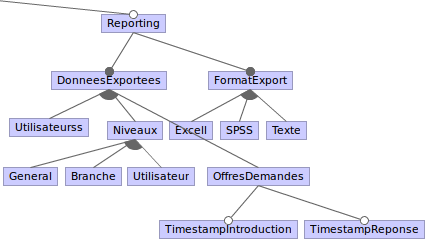
\includegraphics[scale=0.5]{Reporting.png}}
\end{center}

% ================= 60 ===========
\item [Reporting]
\underline{Déf. :}  Le reporting représente un sytème de statistiques offrant des informations sur les données encodées dans le système.  
\\ \underline{Justif. :}  Ce feature peut être présent et utile pour se rendre compte de l'utilisation du site mais n'est pas essentiel.
\newline

\item [DonneesExportees]
\underline{Déf. :}  On retrouve ici les différentes informations qui sont accessibles via le système de de reporting/statistiques
\\ \underline{Justif. :}  Ce feature est obligatoire car un système de reporting sans données exportées n'aurait pas de sens.  3 features sont possibles : l'export de données liées aux utilisateurs,  de celles des transactions ainsi que le niveau hierarchique que l'on désire couvrir.  Il est nécessaire d'en intégrer au moins 1 afin d'avoir des données à exporter.  

\item [Utilisateurs]
\underline{Déf. :}  Un des types de données qu'il peut être possible d'exporter concerne les utilisateurs.
\\ \underline{Justif. :}  Ce feature peut être utile afin de connaitre le public qui fréquente l'outil.
\newline

\item [Niveaux]
\underline{Déf. :}  On définit ici une portée des données qui seront exportées.  C'est à dire que l'on peut vouloir récolter des données issues de diffférentes parties de l'application.
\\ \underline{Justif. :}  Si ce feature est inclu et qu'au moins un des deux autres (utilisateurs ou offres/demandes),  alors le niveau définira l'origine des donées.  Si seuls les niveaux sont inclsu dans les données à exporter,  alors il s'agira d'inforamtions génériques sur ces niveaux.  
\newline

\item [General - Branche - Utilisateur]
\underline{Déf. :}  Ces trois niveaux signifient que l'on récolte des données qui concernent,  respectivement,  tout l'outil,  seulement une zone géographique limitée de l'outil ou uniquement les informations liées à un utilisateur précis.
\\ \underline{Justif. :}  Chaque niveau peut être utile pour analyser l'utilisation de l'outil.
\newline

\item [OffresDemandes]
\underline{Déf. :}  Les données concernant les offres et demandes concernent,  dans le cadre de cette analyse,  l'efficacité du système en terme de temps de réponse pour répondre aux besoins des utilisateurs.  
\\ \underline{Justif. :}  Pour analyser le temps de réponse par rapport aux transactions,  il est nécessaire de pouvoir retrouver le moment où la proposition de transaction a été introduite et où elle a été résolue si un système d'historique est mis en place.  
\newline

\item [TimestampIntroduction - TimestampReponse]
\underline{Déf. :}  Il s'agit,  ici,  du jour et de l'heure auxquels la transaction a d'abord été introduite puis résolue.
\\ \underline{Justif. :}  Ces 2 features sont fondamentalement optionnels mais si on désire pouvoir calculer le temps de réponse,  alors les deux dates et heures sont obligatoires.
\newline

% ================= 70 ===========
\item [FormatExport]
\underline{Déf. :}  Le format d'export correspond au type de support qui contient les données exportées.
\\ \underline{Justif. :}  Si des données peuvent être exportées,  alors il faut définir quel support sera utilisé.  Ce feature est donc obligatoire.
\newline

\item [Excell]
\underline{Déf. :}  Le support excell correspond à un fichier de type "classeur",  ou "tableur".  Typiquement,  un fichier dont l'extension peut être .xls,  .xlsx,  .csv,  ou encore .ods pour la version open-office.  Les fichiers respecteront bien sur les conventions liées à ces formats standardisés.
\\ \underline{Justif. :}  L'export au format excell peut être pratique pour une analyse de base via des graphiques se basant sur les données exportées.  Ce support est assez répandu mais reste limité pour un usage statistique avancé.   Plusieurs formats peuvent cohabiter dans le même outil.
\newline

\item [SPSS]
\underline{Déf. :}  SPSS\copyright est un logiciel de statistiques permettant une analyse plus avancée que les logiciels de bureautique de type "classeur".
\\ \underline{Justif. :}  Un export au format SPSS est intéressant pour alimenter les analyses réalisées dans le cadre d'études,  par exemple,  à la VUB.
\newline

\item [Texte]
\underline{Déf. :}  Le format texte est le plus simple.  Il correspond à un simple fichier sans structure standardisée.   Il est tout de même important de bien caractériser les données reprises.
\\ \underline{Justif. :}  Ce format est le plus simple et le plus facile à mettre en place mais offre moins de possibilités et facilités pour l'utilisation des données dans le futur.
\newline

\begin{center}
\fbox{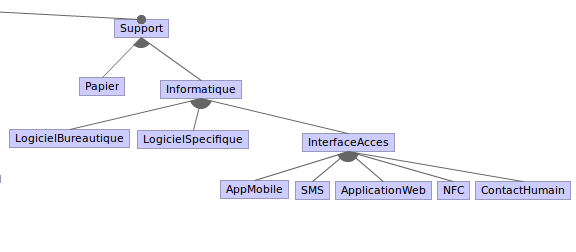
\includegraphics[scale=0.5]{Support.png}}
\end{center}

\item [Support]
\underline{Déf. :}  Ce feature désigne le support technique utilisé par l'outil.
\\ \underline{Justif. :}  Si un outil existe,  alors il doit avoir au moins 1 support pour exister.  Ce feature est donc obligatoire et au moins 1 des fils doit être inclus.
\newline

\item [Papier]
\underline{Déf. :}  Le support papier est le plus simple à mettre en place mais certainement le moins efficace.  Il implique qu'une personne centralise tous les documents.
\\ \underline{Justif. :}  Certaines organisations fonctionnent de la sorte,  souvent pour raison historiques.  Il peut s'agit,  par exemple,  d'un petit groupe de personnes et qui peut avoir grandi mais n'a pas changé d'outil.
\newline

\item [Informatique]
\underline{Déf. :}  Une manière plus efficace de s'organiser de nos jours passe par l'informatique,  au sens ethymologique du terme,  c'est-à-dire le traitement automatique des informations.  Plusieurs supports existent pour ce traitement automatisé.
\\ \underline{Justif. :}  Développer une solution informatique pour un outil de gestion est un investissement initial en temps (et souvent argent) assez conséquent mais rapidement rentabilisé si la solution est appropriée.  Remarquons que l'informatique fait gagner beaucoup de temps quand cela fonctionne comme prévu mais en fait perdre beaucoup dans le cas contraire.
\newline

\item [LogicielBureautique]
\underline{Déf. :}  Ce feature représente l'utilisation d'un logiciel tel que ceux des suites de bureautique (Microsoft Office \copyright ou OpenOffice).  On peut ainsi utiliser un tableur ou un système de gestion de base de données.
\\ \underline{Justif. :}  Ce type de logiciel est une bonne première approche d'un outil de gestion informatisée mais possède ses limites d'efficacité.
\newline

\item [LogicielSpecifique]
\underline{Déf. :}  Un logiciel spécifique est un logiciel développé dans le but de gérer une organisation telle que les économies d'échange local.  
\\ \underline{Justif. :}  Des exemples de ce type de logiciels ont été cités dans l'explication du problème (\ref{autresOrgas}).  
\newline

\item [InterfaceAcces]
\underline{Déf. :}  Ce feature regroupe les moyens techniques permettant d'accéder aux fonctionnalités de l'outil.
\\ \underline{Justif. :}  Plusieurs moyens peuvent coexister pour accéder à l'outil mais il en faut au minimum 1 sinon l'outil n'en est pas un.
\newline

% ================= 80 ===========
\item [AppMobile]
\underline{Déf. :}  Ce feature regroupe la possibilité d'accéder à l'outil via une application développée pour les smartphones ou tablettes ainsi que les sites web développés pour s'adapter aux smartphones et autres supports du même type.  
\\ \underline{Justif. :}   Ce type d'accès est utile pour augmenter l'interactivité avec les utilisateurs et peut,  par exemple,  permettre d'avoir des fonctionnalités de localisation par rapport au lieu encodé pour la transaction.
\newline

\item [SMS]
\underline{Déf. :}  Certaines fonctionnalités peuvent être accessibles via des SMS,  comme par exemple la validation d'une transaction dès que celle-ci est terminée.
\\ \underline{Justif. :}  Ce type d'interface peut aussi permettre plus d'interactivité avec les utilisateurs mais reste assez limitée en terme de fonctionnalités puisque les SMS se résument à des messages uniquement textuels. 
\newline

\item [ApplicationWeb]
\underline{Déf. :}  L'interface la plus répandue est l'interface web "classique".   On retrouve ici les applications web accessibles depuis un navigateur internet.  
\\ \underline{Justif. :}  Ce feature est certainement le plus commun à implémenter et utiliser et donc,  peut-être,  un choix de première interface de base.
\newline

\item [NFC]
\underline{Déf. :}  NFC signifie Near Field Communication.  Cette technologie consiste à une communication entre 2 appareils.  L'idée de base est similaire à la technologie bluetooth.
\\ \underline{Justif. :}  Cette technologie est en cours de développement pour l'application QOIN (\ref{QOIN}).  Cela peut être utile pour valider des transactions entre 2 acteurs lors de la rencontre physique de ceux-ci.
\newline

\item [ContactHumain]
\underline{Déf. :}  De nos jours,  on utilise beaucoup d'outils pour communiquer mais n'oublions pas les bases : un contact humain.  Ainsi on peut considérer que l'utilisateur peut utiliser l'outil via la rencontre avec une personne gérant l'outil.  
\\ \underline{Justif. :}  Cette possibilité est à prendre en compte car si le feature est inclus,  cela peut avoir un impact sur les méthodes d'administration possibles.  Le projet BuurtPensioen fait partie de ceux qui intègrent cette possibilité via des permanences par exemple.  
\newline

\begin{center}
\fbox{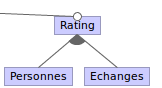
\includegraphics[scale=0.5]{Rating.png}}
\end{center}

\item [Rating]
\underline{Déf. :}  Le rating est un système qui permet de donner une note d'appréciation sur certains éléments de l'outil.
\\ \underline{Justif. :}  Ce feature peut être utile afin,  par exemple,  d'amener une certaine auto-régulation dans l'outil.
\newline

\item [Personnes]
\underline{Déf. :}  Un rating sur les personnes implique que l'on puisse commenter ou noter de façon quantitative un acteur de l'outil.  Ceci met alors en place un concept de "réputation" des acteurs.
\\ \underline{Justif. :}  Ce feature peut être une seconde façon d'amener de la sécurité en plus ou à coté du système de "type de profil" tel que cela existe pour le projet BuurtPensioen.
\newline

\item [Echanges]
\underline{Déf. :}  Un rating sur les échanges implique que l'on puisse commenter ou noter quantitativement une transaction.  De nouveau,  ceci peut permettre à d'autres utilisateurs de voir comment se passent les transactions avec les acteurs impliqués dans l'échange noté.
\\ \underline{Justif. :}  Ceci peut être utile d'un coté pour les utilisateurs mais également pour les gestionnaires afin d'évaluer la qualité des échagnes qui se déroulent via l'outil.
\newline

\end{description}

\subsubsection{Règles de composition}

Nous allons ici décrire les contraintes de composition du schéma.   Ces contraintes doivent être respectées pour obtenir un framework instancié fonctionnel.  Certaines sont plutôt d'ordre "philosophique",  c'est-à-dire qu'elles décrivent une contrainte pour qu'une instanciation soit cohérente.  D'autres sont d'ordre technique,  c'est-à-dire qu'il n'est pas possible d'instancier et programmer le modèle si on ne respecte la règle.

\underline{BusinessUnits > Biens/Objets REQUIRES Monnaie > Temps : } Cette règle  signifie que cela n'a pas de sens d'échanger des objets matériels contre du temps.  Par contre,  une monnaie alternative peut être définie et utilisée.

\underline{GestionEchanges > chaque fils REQUIRES ModeleOffreDemande > le même fils présent : }  Cette règle est d'ordre technique.  Si,  par exemple,  si on désire qu'un administarteur puisse gérer une description d'une offre,  alors le système doit permettre d'encoder des descriptions d'offres.  Ceci s'applique pour chacun des fils. 

\underline{TypesUtilisateurs > chaque fils REQUIRES PublicCible > les mêmes fils présents : }  Cette contrainte est d'ordre philosophique et souligne que les utilisateurs qui s'enregistrent dans le système doivent faire partie du public cible de l'économique qui l'utilise.

\underline{Reporting > Niveaux > Utilisateurs REQUIRES Utilisateurs : }  Cette règle technique spécifie qu'il n'est pas possible d'avoir de statistiques par niveau si l'application ne possède pas cet élément de  hierarchie.

\underline{Rating > Personnes REQUIRES Utilisateurs : }  De même,  il n'est pas possible d'attribuer des appréciation aux comptes des utilisateurs si le système ne permet pas de créer des comptes.

\underline{Reporting REQUIRES Support > Informatique : } Pour que des statistiques puissent être faites,  il est nécessaire d'avoir un support informatique.  

\underline{Support > Informatique > Interface > Contact Humain REQUIRES Administration : }  Cette règle souligne que pour pouvoir intéragir avec le système au nom d'une tierce personne,  il faut pouvoir usurper son identité et donc utiliser un "mode administrateur".  

\underline{Administration > Gestion Profils REQUIRES Utilisateurs : } Cette contrainte souligne qu'il n'est pas possible de gérer des profils si le système n'offre pas de système de comptes d'utilisateur.

\subsubsection{Le feature model de Buurtpensioen}

Maintenant que le modèle des features est défini,  nous allons l'instancier au cas de Buurtpensioen,  et plus particulièrement à la solution proposée par le groupe d'étudiants,  afin de vérifier que le modèle est correct.

$\vcenter{\hbox{\fbox{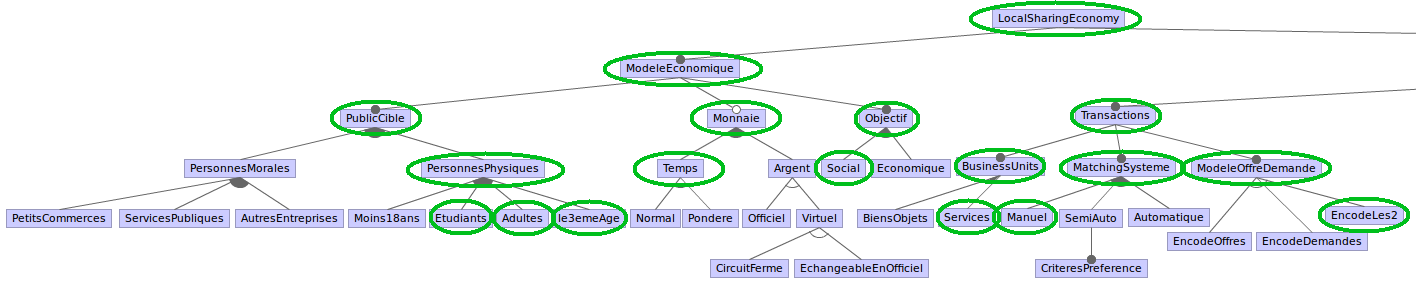
\includegraphics[scale=0.38,angle=90]{BP1.png} } }}$ \hspace{3 cm}
$\vcenter{\hbox{\fbox{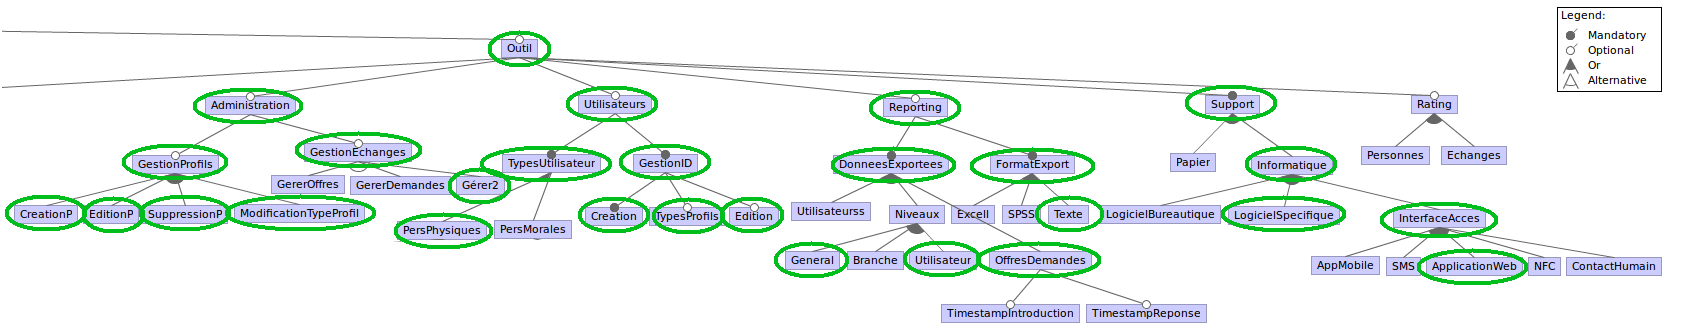
\includegraphics[scale=0.38,angle=90]{BP2.png} } }}$
